\begin{frame}
	\frametitle{Motivation}
	\only<1,2,4,6> {
		\begin{itemize}
			\item<1-> Kürzeste Rundreise finden.
			      \begin{itemize}
				      \item<2-> 	Handlungsreisende
				      \item<4-> 	Computerchips
			      \end{itemize}
		\end{itemize}}
	\only<3> {
		\begin{figure}
			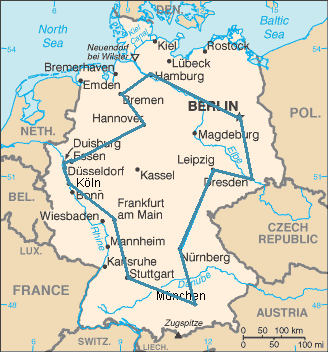
\includegraphics[scale=0.4]{images/TSP_Deutschland_3.png}
			\caption{Optimaler Reiseweg eines Handlungsreisenden durch die 15 größten Städte Deutschlands. Die angegebene Route ist die kürzeste von 43.589.145.600 möglichen.}
		\end{figure}
	}
	\only<5>{
		\begin{figure}
			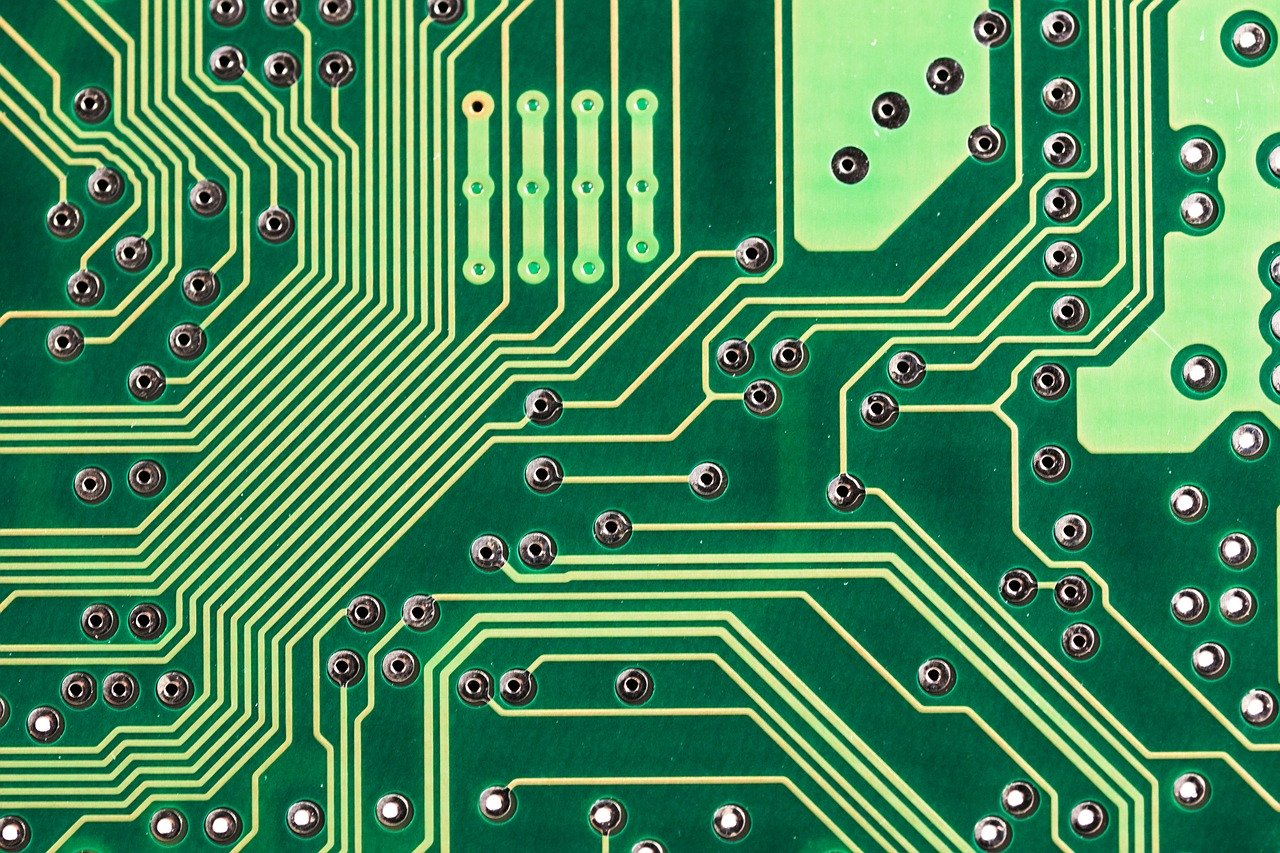
\includegraphics[scale=0.17]{images/computer-chip.jpg}
			\caption{Ein großer Teil des Aufwands beim Erstellen vom Computerchips entfällt auf Optimierung, z.B. auch die kürzeste Route zum Bohren zu finden.}
		\end{figure}
	}
\end{frame}